\subsection{Elastisk net}
I dette afsnit introduceres en shrinkage metode kaldet elastisk net, som kombinerer ridge regression og lasso.
Metoden blev først præsenteret af \citep{zou_hastie}.

Selvom lasso har vist succes i mange tilfælde, har den også nogle begrænsninger:
%
\begin{enumerate}[label=\textnormal{(\arabic*)}]
    \item Hvis $p>n$, da udvælger lasso højst $n$ variable, eftersom lasso er et konvekst optimeringsproblem (KAN DET BEVISES). Derudover er lasso ikke veldefineret medmindre \(\Vert \beta \Vert_1 \leq t\). \label{itm:1}
    \item Hvis der eksisterer en gruppe af variable, som har høj parvis korrelation, da har lasso en tendens til blot at udvælge  én variabel fra denne gruppe og denne variabel udvælges tilfældigt (MÅSKE EKS PÅ DET). \label{itm:2}
    \item Hvis $n>p$ og variablerne er korrelerede, da er det empirisk bevist at prædiktions performance af lasso er domineret af ridge regression \citep{lasso}.  \label{itm:3}
\end{enumerate}
%
Målet er at finde en metode som overkommer ovenstående begrænsninger.
Ridge regression kan håndterer multikollinaritet, da den averages effekten af mutually korrelerede variable.
Men somsagt giver ridge regression ikke en sparse løsning.

Antag responsvariablen er centreret og prediktorerne er standardiseret, da er det naive elastiske net givet ved
\begin{align}
\arg \min_{\beta} \cbr{ \frac{1}{2n} \Vert \y - \X \beta \Vert_2^2 + \lambda_1 \Vert \beta \Vert_2^2 + \lambda_2 \Vert \beta \Vert_1}, \label{eq:EN1}
\end{align}
for \(\lambda_1, \lambda_2 \geq 0\).
Lad \(\alpha = \frac{\lambda_1}{\lambda_1 + \lambda_2}\), da kan \eqref{eq:EN1} omskrives til følgende
\begin{align*}
\arg \min_{\beta} \cbr{\frac{1}{2n} \Vert \y - \X \beta \Vert_2^2}, \ \text{underlagt at } \del{1-\alpha} \Vert \beta \Vert_2^2 + \alpha \Vert \beta \Vert_1 \leq t,
\end{align*}
som på Lagrange form er givet ved
\begin{align}
\arg \min_{\beta} \cbr{\frac{1}{2n} \Vert \y - \X \beta \Vert_2^2 + \lambda \sbr{(1- \alpha) \Vert \beta \Vert_2^2 + \alpha \Vert \beta \Vert_1}}. \label{eq:4.2}
\end{align}
Hvis $\alpha=1$, da reduceres strafleddet til $\ell_1$-normen svarende til strafleddet for lasso, og hvis $\alpha=0$ reduceres det til den kvadrerede $\ell_2$-norm svarende til strafleddet for ridge regression.
Optimeringsproblemet  \eqref{eq:4.2} er streng konveks for \(\alpha \in [0,1)\), hvilket betyder, at der eksisterer en entydig løsning uafhængigt af korrelationsstrukturen af $\X$.
For  \(\alpha=1\) er problemet konveks, men ikke streng konveks.
Dette ses tydeligt på figur \ref{fig:elastisk}.
%
\begin{figure}[H]
\centering
\scalebox{0.8}{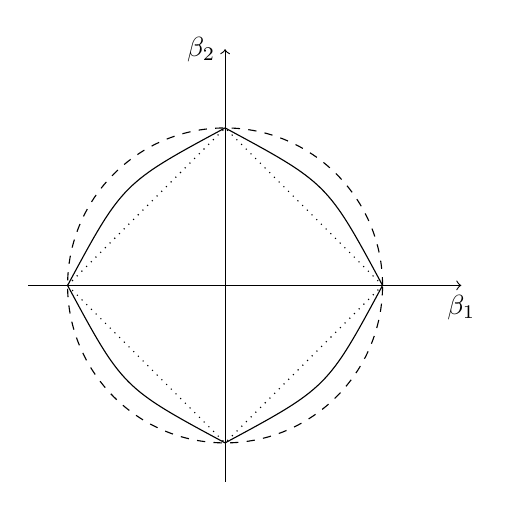
\begin{tikzpicture}
\draw[dashed] (0,0) circle (2cm);
\draw[dotted] (-2,0) -- (0,-2) -- (2,0) -- (0,2) -- (-2,0); 
\draw (-2,0) .. controls (-1.3,1.3) .. (0,2);
\draw (0,2) .. controls (1.3,1.3) .. (2,0);
\draw (-2,0) .. controls (-1.3,-1.3) .. (0,-2);
\draw (0,-2) .. controls (1.3,-1.3) .. (2,0);
\draw [<-] (0,3) node [left] {$\beta_2$}-- (0,-2.5);
\draw[<-] (3,0) node [below] {$\beta_1$} -- (-2.5,0);
\end{tikzpicture}}
\caption[optional short text]{To dimensional illustration af betingelsesområderne for shrinkage metoderne: \tikz[baseline]{\draw[dashed] (0,.5ex)--++(.5,0) ;} ridge regression,  \tikz[baseline]{\draw[dotted] (0,.5ex)--++(.5,0) ;} lasso og \tikz[baseline]{\draw (0,.5ex)--++(.5,0) ;} elastisk net med \(\alpha = 0.5\). Vi observerer at singulariteten i hjørnerne og kanterne er streng konveks. Styrken af konveksitet varierer med \(\alpha\).} \label{fig:elastisk}
\end{figure}
%
En tre dimensionel illustration af betingelsesområderne for det elastiske net og standard lasso er givet på figur \ref{fig:elastisk_net}.
Heraf ses at det elastiske net har egenskaberne af både $\ell_1$ kuglen og $\ell_2$ kuglen: de skarpe hjørner og kanter opfordrer til variable udvælgelse, mens de kurvede konturer opfordrer stærk korreleret variable til at dele koefficienter.
%
\begin{figure}[H]
\centering
 \scalebox{0.5}{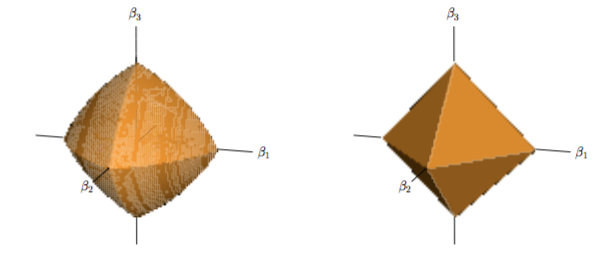
\includegraphics{fig/elastisk_net.jpg}}
\caption{Kuglen for elastisk net med \(\alpha=0.7\) (venstre) og \(\ell_1\) kuglen (højre) for tre variable.}
\label{fig:elastisk_net}
\end{figure}
%
Det viser sig, at optimeringsproblemet for naive elastisk net kan transformeres til et ækvivalent lasso problem på augmented data.
%
\begin{lem} \label{lem:elastisk_net}
Givet data \(\del{\y, \X}\) og parametrene \(\del{\lambda_1, \lambda_2}\), defineres et augmented datasæt 
\begin{align*}
\X^* = \del{1 + \lambda_1}^{-1/2} \begin{bmatrix}
\X \\ \sqrt{\lambda_1} \mathbf{I}
\end{bmatrix}, \quad \y^* = \begin{bmatrix}
\y \\ \mathbf{0}
\end{bmatrix},
\end{align*}
hvor \(\X^* \in \mathbb{R}^{\del{n+p} \times p}\) og \(\y^* \in \mathbb{R}^{n+p}\).
Lad \(\gamma = \frac{\lambda_2}{\sqrt{1+\lambda_1}}\) og \(\beta^* = \sqrt{1+\lambda_1} \beta\), da kan \eqref{eq:EN1} omskrives til
\begin{align*}
\hat{\beta}^* = \arg \min_{\beta^*} \cbr{\frac{1}{2n} \Vert \y^* - \X^* \beta^* \Vert_2^2 +\gamma \Vert \beta^* \Vert_1},
\end{align*}
og
\begin{align*}
\hat{\beta}^\text{naivEN} = \frac{1}{\sqrt{1+\lambda_1}} \hat{\beta}^*.
\end{align*}
\end{lem}
%
Da \(\X^*\) har rang \(p\), kan metoden i princippet altid vælge alle \(p\) prediktorer.
Dermed er naiv elastisk net ikke begrænset til blot at vælge \(n\) prediktorer hvis \(p > n\), som er tilfældet for lasso som beskrevet i \ref{itm:1}.
Lemma \ref{lem:elastisk_net} viser også, at naiv  elastisk net udfører variabel udvælgelse svarende til lasso.
%
\begin{exmp}
Hvis \(\X\) er ortogonal, da er \(\hat{\beta}^\text{OLS} = \X^T \y\) og der gælder, at
\begin{align*}
\hat{\beta}^\text{ridge} &= \frac{\hat{\beta}^\text{OLS}}{1+\lambda_1} \\
\hat{\beta}^\text{lasso} &= \text{sign} \del{\hat{\beta}_i^\text{OLS}} \del{\left\vert \hat{\beta}_i^\text{OLS} \right\vert - \frac{\lambda_2}{2}}_+ \\
\hat{\beta}^\text{naivEN} &= \text{sign} \del{\hat{\beta}_i^\text{OLS}} \frac{\del{\left\vert \hat{\beta}_i^\text{OLS} \right\vert - \frac{\lambda_2}{2}}_+}{1+\lambda_1}
\end{align*}
Figur \ref{fig:elastisk2} viser de operationelle egenskaber af ridge regression, lasso og naiv elastisk net, hvis \(\X\) er ortogonal. Heraf ses det også at naiv elastisk net er en two-stage procedure, først har vi en ridge lignende shrinkage som efterfølges af en lasso lignende thresholding.
%
\begin{figure}[H]
\centering
\scalebox{0.8}{\begin{tikzpicture}
\draw[loosely dotted] (-3,-3) -- (3,3);
\draw[dotted] (-3,-2) -- (3,2);
\draw (-3,-1.5) -- (-0.75,0) -- (0.75,0) -- (3,1.5);
\draw[dashed] (-3,-2.2) -- (-0.75,0) -- (0.75,0) -- (3,2.2); 
\draw [<-] (0,3.5) node [left] {$\widehat{\beta}$}-- (0,-3.5);
\draw[<-] (3.5,0) node [below] {$\beta$} -- (-3.5,0);
\end{tikzpicture}
}
\caption[optional short text]{Eksakte løsninger for \tikz[baseline]{\draw[dotted] (0,.5ex)--++(.5,0) ;} ridge regression, \tikz[baseline]{\draw[dashed] (0,.5ex)--++(.5,0) ;} lasso og \tikz[baseline]{\draw (0,.5ex)--++(.5,0) ;} naiv elastisk net, hvis \(\X\) er ortogonal med \tikz[baseline]{\draw[loosely dotted] (0,.5ex)--++(.5,0) ;} OLS for parametrene \(\lambda_1=1\) og \(\lambda_2=2\).} \label{fig:elastisk2}
\end{figure}
%
\end{exmp}
%
Hvis vi har en gruppe af højt korreleret variable, da vil lasso blot udvælge én variable og den udvælges tilfældigt, som nævnt i \ref{itm:2}.
Men elastisk net udvælger alle variable i denne gruppe, som vi nu vil vise. 
En regression metode udviser denne evne, hvis regressions koeffcienterne af en gruppe af højt korreleret variable er approksimativt ens.

\begin{thm} \label{thm:elastisk_net}
Givet data \(\del{\y, \X}\) og parametrene \(\del{\lambda_1, \lambda_2}\), hvor responsvariablen er centreret og prediktorerne er standardiseret.
Lad \(\hat{\beta} \del{\lambda_1, \lambda_2}\) være estimatet for naiv elastisk net.
Antag \(\hat{\beta}_i \del{\lambda_1, \lambda_2} \hat{\beta}_j \del{\lambda_1, \lambda_2} > 0\).
Definer
\begin{align*}
D_{\lambda_1, \lambda_2} \del{i,j} = \frac{1}{\Vert \y \Vert_1} \vert \hat{\beta}_i \del{\lambda_1, \lambda_2} - \hat{\beta}_j \del{\lambda_1, \lambda_2} \vert,
\end{align*}
da er
\begin{align}
D_{\lambda_1, \lambda_2} \del{i,j} \leq \frac{1}{\lambda_1} \sqrt{2 \del{1-\rho}}, \label{eq:EN5}
\end{align}
hvor \(\rho = \mathbf{x}_i^T \mathbf{x}_j\) er den empiriske korrelation.
\end{thm}
\begin{proof}
Hvis \(\hat{\beta}_i \del{\lambda_1, \lambda_2} \hat{\beta}_j \del{\lambda_1, \lambda_2} > 0\), da er både \(\hat{\beta}_i \del{\lambda_1, \lambda_2}\) og \(\hat{\beta}_j \del{\lambda_1, \lambda_2}\) ikke-nul og der må gælder, at \(\text{sign} \cbr{\hat{\beta}_i \del{\lambda_1, \lambda_2}} = \text{sign} \cbr{\hat{\beta}_j \del{\lambda_1, \lambda_2}}\).
Lad \(L \del{\lambda_1,\lambda_2, \beta} = \frac{1}{2n} \Vert \y - \X \beta \Vert_2^2 + \lambda_1 \Vert \beta \Vert_2^2 + \lambda_2 \Vert \beta \Vert_1\), således at  \(\arg \min_{\beta} \cbr{L \del{\lambda_1,\lambda_2, \beta}}\) svarer til \eqref{eq:EN1}.
Da må \(\hat{\beta} \del{\lambda_1, \lambda_2}\) opfylde, at
\begin{align*}
\frac{\partial L \del{\lambda_1,\lambda_2, \beta} }{\partial \beta_k} \mid_{\beta = \hat{\beta} \del{\lambda_1, \lambda_2}}=0, \text{ hvis } \hat{\beta}_k \del{\lambda_1, \lambda_2} \neq 0.
\end{align*}
Derfor har vi, at
\begin{align}
-\mathbf{x}_i^T \del{\y - \X \hat{\beta} \del{\lambda_1, \lambda_2}} + 2 \lambda_1 \hat{\beta}_i \del{\lambda_1, \lambda_2} + \lambda_2 \text{sign} \cbr{\hat{\beta}_i \del{\lambda_1, \lambda_2}} &= 0, \label{eq:EN2}\\
-\mathbf{x}_j^T \del{\y - \X \hat{\beta} \del{\lambda_1, \lambda_2}} + 2 \lambda_1 \hat{\beta}_j \del{\lambda_1, \lambda_2} + \lambda_2 \text{sign} \cbr{\hat{\beta}_j \del{\lambda_1, \lambda_2}} &= 0. \label{eq:EN3}
\end{align}
Vi subtraherer \eqref{eq:EN2} fra \eqref{eq:EN3} og finder, at
\begin{align*}
\del{\mathbf{x}_j^T-\mathbf{x}_i^T} \del{\y - \X \hat{\beta} \del{\lambda_1, \lambda_2}} + \lambda_1 \del{\hat{\beta}_i \del{\lambda_1, \lambda_2} - \hat{\beta}_j \del{\lambda_1, \lambda_2}} =0,
\end{align*}
som er ækvivalent med
\begin{align}
\hat{\beta}_i \del{\lambda_1, \lambda_2} - \hat{\beta}_j \del{\lambda_1, \lambda_2} = \frac{1}{\lambda_1} \del{\mathbf{x}_i^T-\mathbf{x}_j^T} \hat{r}\del{\lambda_1, \lambda_2}, \label{eq:EN4}
\end{align}
hvor \(\hat{r}\del{\lambda_1, \lambda_2} = \y - \X  \hat{\beta} \del{\lambda_1, \lambda_2}\) er en vektor af residualer.
Da \(\X\) er standardiseret, har vi, at \(\Vert \mathbf{x}_i - \mathbf{x}_j \Vert_2^2=2 \del{1-\rho}\), hvor \(\rho = \mathbf{x}_i^T \mathbf{x}_j\).
Af \eqref{eq:EN1} må vi have, at
\begin{align*}
L \del{\lambda_1,\lambda_2, \hat{\beta}\del{\lambda_1, \lambda_2}} \leq L \del{\lambda_1,\lambda_2, \beta = 0},  
\end{align*}
dvs
\begin{align*}
\frac{1}{2n} \Vert \hat{r} \del{\lambda_1, \lambda_2} \Vert_2^2 + \lambda_1 \Vert \hat{\beta} \del{\lambda_1, \lambda_2} \Vert_2^2 + \lambda_2 \Vert \hat{\beta} \del{\lambda_1, \lambda_2} \Vert_1 \leq \frac{1}{2n} \Vert \y \Vert_2^2.  
\end{align*}
Dermed er \(\vert \hat{r} \del{\lambda_1, \lambda_2} \vert \leq \vert \y \vert\) og \eqref{eq:EN4} medfører, at
\begin{align*}
D_{\lambda_1, \lambda_2} \del{i,j} \leq \frac{1}{\lambda_1} \frac{\vert \hat{r} \del{\lambda_1, \lambda_2} \vert}{\vert \y \vert} \vert \mathbf{x}_i - \mathbf{x}_j \vert  \leq \frac{1}{\lambda_1} \sqrt{2 \del{1-\rho}}.
\end{align*}
\end{proof}
Mængden \(D_{\lambda_1, \lambda_2} \del{i,j}\) betegner differensen mellem koefficient stierne af prediktor \(i\) og \(j\).
Hvis \(\mathbf{x}_i\) og \(\mathbf{x}_j\) er højt korreleret, dvs \(\rho \approx 1\), giver sætning \ref{thm:elastisk_net}, at differensen mellem koefficient stierne af prediktor \(i\) og \(j\) er næsten 0.
Den øvre grænse i \eqref{eq:EN5} giver en beskrivelse af denne gruppering effekt som naiv elastisk net har??\\[4mm]
%
Empiriske resultater har vist, at naiv elastisk net ikke er tilfredsstillende, medmindre den er tæt på enten ridge regression eller lasso.
Derfor kaldes den \textit{naiv}.
Som nævnt tidligere bestemmes en metodes prediktions performance gennem bias-variance tradeoff. 
Naiv elastisk net er en two-stage procedure. For ethvert fast \(\lambda_1\) finder vi først ridge regression koefficienterne, og derefter shrinkages langs lasso koefficient løsnings stien. Derfor inkluderes en dobbelt shrinkage.
Double shrinkage reducerer ikke variansen meget og introducere unødvendig ekstra bias i forhold til ridge regression eller lasso.
Derfor introduceres blot elastisk net.

I lemma \ref{lem:elastisk_net} fandt vi, at naiv elastisk net løser følgende 
\begin{align}
\hat{\beta}^* = \arg \min_{\beta^*} \cbr{\frac{1}{2n} \Vert \y^* - \X^* \beta^* \Vert_2^2 + \frac{\lambda_2}{\sqrt{1+\lambda_1}} \Vert \beta^* \Vert_1}. \label{eq:EN8}
\end{align}
Estimaterne for elastisk net (korrigeret) er defineret ved
\begin{align*}
\hat{\beta}^\text{EN} = \sqrt{\del{1+\lambda_1}} \hat{\beta}^*.
\end{align*}
Da \(\hat{\beta}^\text{naivEN} = \frac{1}{\sqrt{1+\lambda_1}} \hat{\beta}^*\), har vi, at
\begin{align*}
\hat{\beta}^\text{EN} = \del{1+\lambda_1} \hat{\beta}^\text{naivEN}.
\end{align*}
Dermed er elastisk net koefficienterne faktisk reskaleret naiv elastisk net koefficienter.
Denne transformation bevarer variabel udvælgelsen af naiv elastisk net og er den simpleste måde at annullere det ekstra shrinkage.
Derfor er egenskaberne for naiv elastiske net, som er beskrevet i dette afsnit, stadig gældende for elastisk net.

Et andet længere argument for at vælge \(1+\lambda_1\) som skaleringsfaktor, men det forstår jeg ikke!!!
%
\begin{thm} \label{thm:elastisk_net2}
Givet data \(\del{\y, \X}\) og parametrene \(\del{\lambda_1, \lambda_2}\) da er estimaterne for elastisk net givet ved
\begin{align}
\hat{\beta}^\text{EN} = \arg \min_\beta \cbr{ \frac{1}{2n} \del{\beta^T \del{\frac{\X^T \X + \lambda_1 \mathbf{I}}{1 + \lambda_1}} \beta - 2 \y^T \X \beta} + \lambda_2 \Vert \beta \Vert_1}. \label{eq:EN6}
\end{align}
Estimatoren for lasso kan omskrives til
\begin{align}
\hat{\beta}^\text{lasso} = \arg \min_\beta \cbr{ \frac{1}{2n} \del{ \beta^T \del{\X^T \X} \beta - 2 \y^T \X \beta } + \lambda_2 \Vert \beta \Vert_1}. \label{eq:EN7}
\end{align}
\end{thm}
\begin{proof}
Af ligning \eqref{eq:EN8} har vi, at
\begin{align}
\hat{\beta} &= \arg \min_{\beta} \cbr{\frac{1}{2n} \left\Vert \y^* - \X^* \frac{\beta}{\sqrt{1+\lambda_1}} \right\Vert_2^2 + \frac{\lambda_2}{\sqrt{1+\lambda_1}} \left\Vert \frac{\beta}{\sqrt{1+\lambda_1}} \right\Vert_1} \nonumber \\
&=\arg \min_{\beta} \cbr{\frac{1}{2n} \del{\beta^T \del{\frac{\X^{*^T} \X^*}{1+\lambda_1}} \beta - 2 \frac{\y^{*^T} \X^* \beta}{\sqrt{1+\lambda_1}} + \y^{*^T} \y^*} + \frac{\lambda_2 \Vert \beta \Vert_1}{1+\lambda_1}}. \label{eq:EN9}
\end{align}
Følgende identiteter
\begin{align*}
\X^{*^T} \X^* &= \frac{\X^T \X + \lambda_1 \mathbf{I}}{1+ \lambda_1}, \\
\y^{*^T} \X^* &= \frac{\y^T \X}{\sqrt{1+\lambda_1}} ,\\
\y^{*^T} \y^* &= \y^T \y, 
\end{align*}
indsættes i \eqref{eq:EN9}, og vi får, at
\begin{align*}
\hat{\beta} &= \arg \min_{\beta} \cbr{\frac{1}{2n} \del{\beta^T \del{\frac{\X^T \X + \lambda_1 \mathbf{I}}{\del{1+\lambda_1}^2}} \beta - 2 \frac{\y^T \X \beta}{1+\lambda_1} + \y^T \y} + \frac{\lambda_2 \Vert \beta \Vert_1}{1+\lambda_1}} \\ 
%&= \arg \min_{\beta} \cbr{\frac{1}{2n} \frac{1}{1+\lambda_1} \del{\beta^T \del{\frac{\X^T \X + \lambda_1\mathbf{I}}{1+ \lambda_1}} \beta - 2 \y^T \X \beta + \lambda_2 \Vert \beta \Vert_1} + \y^T \y} \\
&= \arg \min_{\beta} \cbr{ \frac{1}{2n} \del{\beta^T \del{\frac{\X^T \X + \lambda_1\mathbf{I}}{1+ \lambda_1}} \beta - 2 \y^T \X \beta} + \lambda_2 \Vert \beta \Vert_1},
\end{align*}
hvor \(\y^T \y= 0 \).
\end{proof}
%
Sætning \ref{thm:elastisk_net2} fortolker elastisk net som en stabil version af lasso.
Lad \(\hat{\Sigma} = \X^T \X\) være den empiriske korrelationsmatrix og
\begin{align*}
\frac{\X^T \X + \lambda_1 \mathbf{I}}{1 + \lambda_1} = (1-\gamma) \hat{\Sigma} + \gamma \mathbf{I},
\end{align*}
hvor \(\gamma=\frac{\lambda_1}{1+\lambda_1}\) shrinks \(\hat{\Sigma}\) mod identitetsmatricen.
Ligning \eqref{eq:EN6} og \eqref{eq:EN7} viser, at reskalere elastisk net er ækvivalent med at erstatte \(\hat{\Sigma}\) med dens shrunken version i lasso.


Somsagt er lasso et specialtilfælde af elastisk net med \(\lambda_1=0\). 
Et andet interessant specialtilfælde er når \(\lambda_1 \rightarrow \infty\).
Af sætning \ref{thm:elastisk_net2} gælder, at \(\hat{\beta}^\text{EN} \rightarrow \hat{\beta} \del{\infty}\) når \(\lambda_1 \rightarrow \infty\), hvor
\begin{align*}
\hat{\beta} \del{\infty} = \arg \min_\beta \cbr{\frac{1}{2n} \del{\beta^T \beta - 2 \y^T \X \beta} + \lambda_2 \Vert \beta \Vert_1}.
\end{align*}
\(\hat{\beta} \del{\infty}\) har en simpel lukket løsning, som er givet ved
\begin{align*}
\hat{\beta} \del{\infty}_i = \text{sign} \del{\y^T \mathbf{x}_i} \del{\left\vert \y^T \mathbf{x}_i \right\vert - \frac{\lambda_2}{2}}_+
\end{align*}
for \(i = 1, \ldots, p\).
Vi har, at \(\y^T \mathbf{x}_i\) er en univariat regressions koefficient af den \(i\)'te prediktor og \(\hat{\beta} \del{\infty}\) er estimaterne som fås udfra soft thresholding på univariater regressions koefficienter.
En univariat soft thresholding ignorerer afhængighedsstrukturen mellem prediktorerne og behandler dem som uafhængige variable.
Elastisk net er en natur bro imellem bridges og lasso.

\subsubsection{Udregning af elastisk net}
Somsagt er optimeringsproblemet for det naive elastiske net \eqref{eq:4.2} konveks og dermed kan flere optimeringsmetoder anvendes til at løse det.
Coordinate descent er særlig effektiv, og opdateringerne er blot en simpel udvidelse af dem for standard lasso i sektion \ref{sec:lasso_estimatoren}.

Igen centreres prediktorerne \(x_{ij}\), hvoraf den optimale skæring er givet ved \(\hat{\beta}_0=\bar{y}=\frac{1}{n} \sum_{j=1}^n y_j\).
Efter at have løst \(\hat{\beta}_0\), udregnes den optimale vektor \(\hat{\beta}= \del{\hat{\beta}_1, \ldots, \hat{\beta}_p}\).

Coordinate descent opdateringen for $j$'te koefficient er givet ved
\begin{align}
\hat{\beta}_j = \frac{S_{\lambda \alpha} \del{\sum_{i=1}^n r_{ij} x_{ij}}}{\sum_{i=1}^n x_{ij}^2 + \lambda (1-\alpha)}, \label{eq:4.4}
\end{align} 
hvor $S_\mu(z)=\text{sign}(z)(z-\mu)_+$ er soft-thresholding operatoren og $r_{ij}=y_i - \hat{\beta}_0 - \sum_{k \neq j} x_{ik} \hat{\beta}_k$ er den partial residual.
Vi gennemløber opdateringen \eqref{eq:4.4} indtil konvergens.
[Friedman et al (2015)]

Algoritmen LARS-EN kan anvendes til at løse elastisk net, som er baseret på algoritmen LARS af \cite{efron}.
Af lemma \ref{lem:elastisk_net}, ved vi at for ethvert fast \(\lambda_1\) er elastisk net problemet ækvivalent med lasso problemet på augmented data.
Derfor kan LARS algoritmen anvendes direkte til at finde en elastisk net løsningssti.
Bemærk at for \(p \gg n\), har augmented data \(p+n\) observationer og \(p\) variable, hvilket kan forsinket udregningerne.


%
\begin{figure}[H]
\centering
\begin{minipage}{0.4\linewidth}
\scalebox{0.3}{\includegraphics{fig/crime_lasso.png}}
\end{minipage}
\hspace{0.2cm}
\begin{minipage}{0.4\linewidth}
\scalebox{0.3}{\includegraphics{fig/crime_EN.png}}
\end{minipage}
\caption{Koefficientstierne for henholdsvis lasso (ventre) og elastisk net med \(\alpha=0.3\) (højre) plottet imod \(\ell_1\)-normen for crime data.} \label{fig:crime_koef_EN}
\end{figure}
%


\newpage
